%%%%%%%%%%%%%%%%%%%%%%%%%%%%%%%%%%%%%%%%%
% Beamer Presentation
% LaTeX Template
% Version 1.0 (10/11/12)
%
% This template has been downloaded from:
% http://www.LaTeXTemplates.com
%
% License:
% CC BY-NC-SA 3.0 (http://creativecommons.org/licenses/by-nc-sa/3.0/)
%
%%%%%%%%%%%%%%%%%%%%%%%%%%%%%%%%%%%%%%%%%

%----------------------------------------------------------------------------------------
%	PACKAGES AND THEMES
%----------------------------------------------------------------------------------------

\documentclass{beamer}

\mode<presentation> {

% The Beamer class comes with a number of default slide themes
% which change the colors and layouts of slides. Below this is a list
% of all the themes, uncomment each in turn to see what they look like.

%\usetheme{default}
%\usetheme{AnnArbor}
%\usetheme{Antibes}
%\usetheme{Bergen}
%\usetheme{Berkeley}
%\usetheme{Berlin}
%\usetheme{Boadilla}
%\usetheme{CambridgeUS}
%\usetheme{Copenhagen}
%\usetheme{Darmstadt}
%\usetheme{Dresden}
%\usetheme{Frankfurt}
%\usetheme{Goettingen}
%\usetheme{Hannover}
%\usetheme{Ilmenau}
%\usetheme{JuanLesPins}
%\usetheme{Luebeck}
%\usetheme{Madrid}
%\usetheme{Malmoe}
%\usetheme{Marburg}
%\usetheme{Montpellier}
%\usetheme{PaloAlto}
%\usetheme{Pittsburgh}
%\usetheme{Rochester}
%\usetheme{Singapore}
%\usetheme{Szeged}
%\usetheme{Warsaw}

% As well as themes, the Beamer class has a number of color themes
% for any slide theme. Uncomment each of these in turn to see how it
% changes the colors of your current slide theme.

%\usecolortheme{albatross}
%\usecolortheme{beaver}
%\usecolortheme{beetle}
%\usecolortheme{crane}
\usecolortheme{dolphin}
%\usecolortheme{dove}
%\usecolortheme{fly}
%\usecolortheme{lily}
%\usecolortheme{orchid}
%\usecolortheme{rose}
%\usecolortheme{seagull}
%\usecolortheme{seahorse}
%\usecolortheme{whale}
%\usecolortheme{wolverine}

%\setbeamertemplate{footline} % To remove the footer line in all slides uncomment this line
%\setbeamertemplate{footline}[page number] % To replace the footer line in all slides with a simple slide count uncomment this line

%\setbeamertemplate{navigation symbols}{} % To remove the navigation symbols from the bottom of all slides uncomment this line
}
\addtobeamertemplate{navigation symbols}{}{%
    \usebeamerfont{footline}%
    \usebeamercolor[fg]{footline}%
    \hspace{1em}%
    \insertframenumber/\inserttotalframenumber
}
% \usepackage[dvipsnames]{xcolor}
\usepackage{xcolor}
\definecolor{mygray}{gray}{0.6}
\usepackage{graphicx} % Allows including images
\usepackage{booktabs} % Allows the use of \toprule, \midrule and \bottomrule in tables
\usepackage{multirow}
\usepackage{comment}

%----------------------------------------------------------------------------------------
%	TITLE PAGE
%----------------------------------------------------------------------------------------

\title[Meta Analysis]{Conditional Cash Transfers and School Attendance:\\A Meta-Analytical Approach} % The short title appears at the bottom of every slide, the full title is only on the title page

\author{Tinghuan Liu\and Oliver Pedrini \and Wenjie Tu} % Your name
\institute[UZH] % Your institution as it will appear on the bottom of every slide, may be shorthand to save space
{
Department of Economics, University of Zurich \\ % Your institution for the title page
\medskip
% \textit{wenjtu@student.ethz.ch} % Your email address
}
\date{November 23, 2021} % Date, can be changed to a custom date

\begin{document}

\begin{frame}
\titlepage % Print the title page as the first slide
\end{frame}


%----------------------------------------------------------------------------------------
%	PRESENTATION SLIDES
%----------------------------------------------------------------------------------------

%------------------------------------------------
%\section{First Section} % Sections can be created in order to organize your presentation into discrete blocks, all sections and subsections are automatically printed in the table of contents as an overview of the talk
%------------------------------------------------

%\subsection{Subsection Example} % A subsection can be created just before a set of slides with a common theme to further break down your presentation into chunks

%------------------------------------------------
%\section{Motivation}


\begin{comment}


\begin{frame}{Helpful?}
    \begin{itemize}
    \item Many empirical studies on the relation between CCT programs and school attendance.\\
    --- Most find \textit{positive} effect
    \bigskip
    \pause
    \\ In this paper: 
    \item Systematically summarizing existing studies through meta-analysis
    \item Heterogeneity of the different studies? 
    \item Publication bias?
    \end{itemize}
\end{frame}

\end{comment}


%\begin{frame}{Meta-Analysis Results Preview}
%\begin{itemize}
%    \item Still find significantly \textit{positive} relation between CCT programs and school attendance.
%    \begin{itemize}
%        \item Fixed-effects model: 2 percentage points
%        \item Random-effects model: 4 percentage points
%    \end{itemize}
%    \pause
%    \bigskip
%    \item An important amount of between-study heterogeneity
%    \pause
%    \bigskip
%    \item No strong evidence of publication bias

%\end{itemize}
    
%\end{frame}


%\begin{frame}
%\frametitle{Overview} % Table of contents slide, comment this block out to remove it
%\tableofcontents % Throughout your presentation, if you choose to use \section{} and \subsection{} commands, these will automatically be printed on this slide as an overview of your presentation
%\end{frame}

%------------------------------------------------


\begin{frame}
\frametitle{Motivation}
Education is important in developing process
\begin{itemize}
    \item Human capital accumulation \textcolor{mygray}{Duflo (2004)}
    \item Avoiding poverty transmission across generations \textcolor{mygray}{Tilak (2002)}.
    \item Technological progress and economic growth \textcolor{mygray}{Barro (2001) and Krueger and Lindahl (2001)}
\end{itemize}
\pause
\bigskip
\bigskip
However, the school attendance is still low in developing countries. 

\end{frame}

\begin{frame}
    \begin{figure}
        \centering
        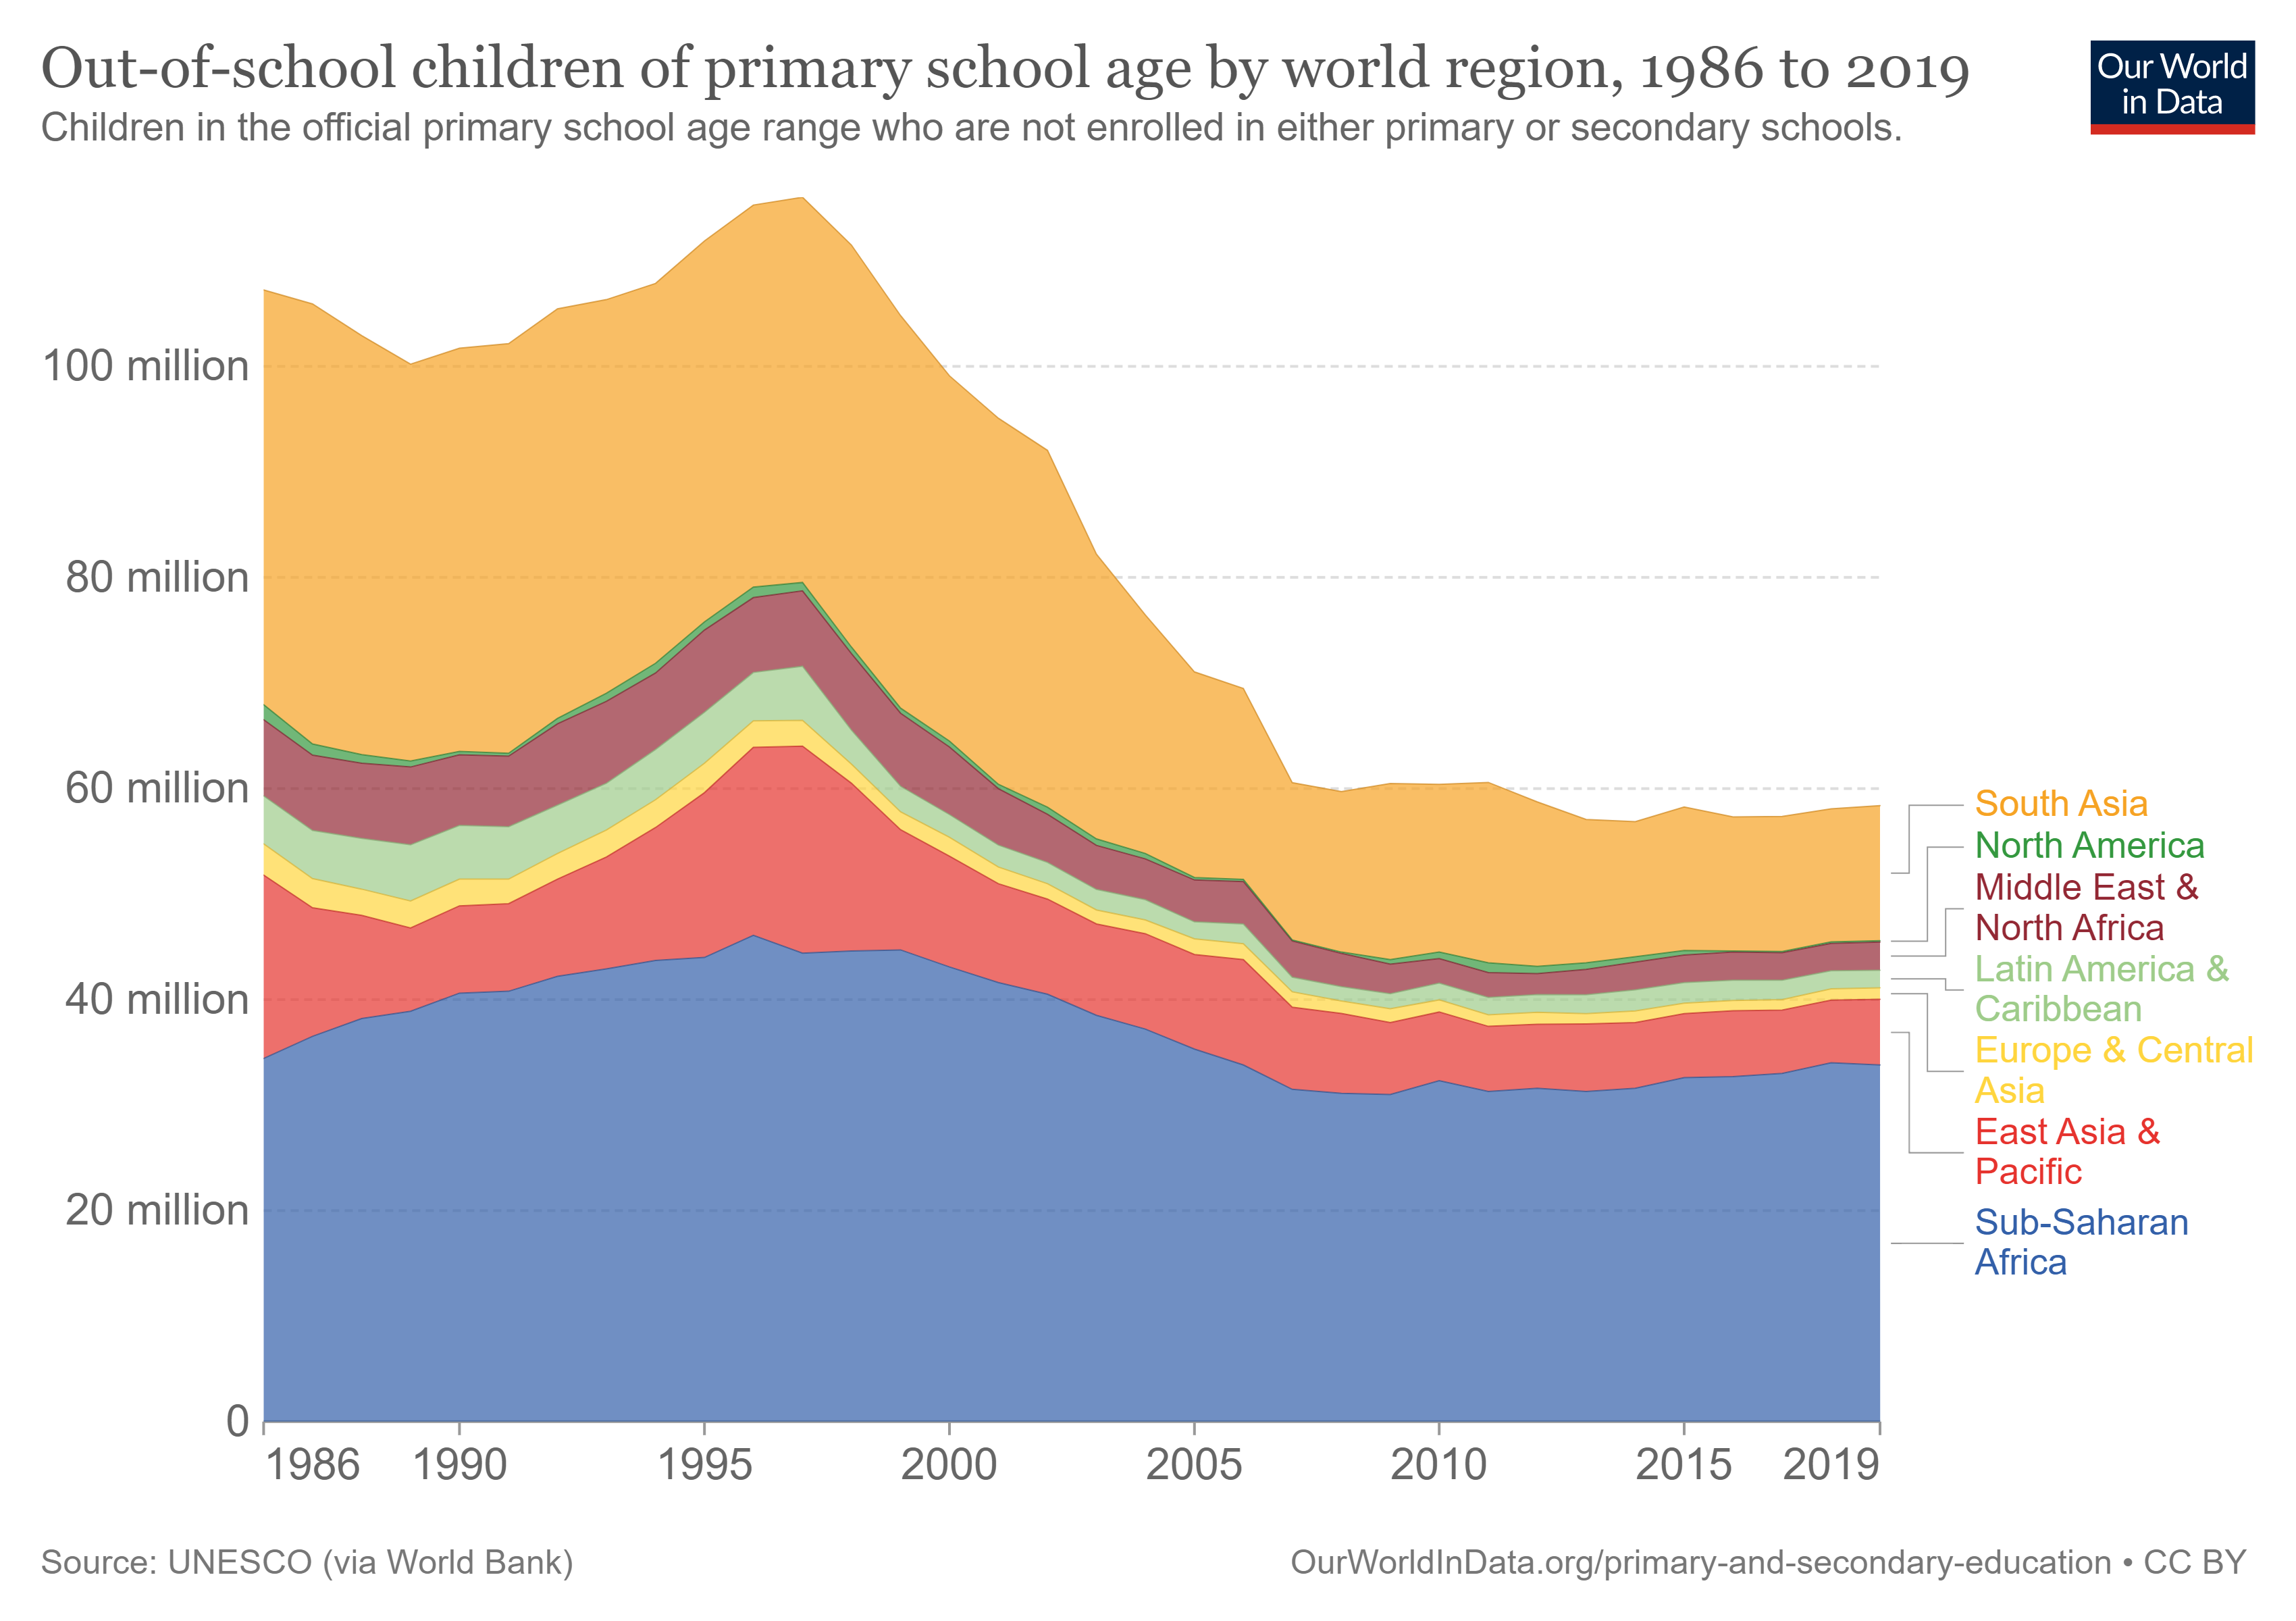
\includegraphics[scale=0.08]{images/out-of-school.png}
        \label{fig:out-of-school}
    \end{figure}
\end{frame}


\begin{frame}{Why?}
    \begin{itemize}
        \item Liquidity constraint + Perceived low returns on education by the parents \textcolor{mygray}{Baland and Robinson (2000) and Kremer and Holla (2009)}
    \end{itemize}
    %\pause
    \begin{figure}
        \centering
        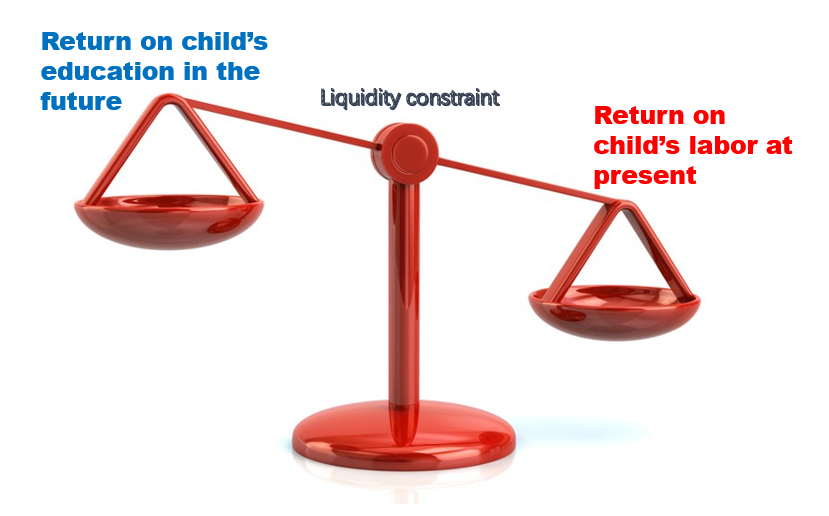
\includegraphics[scale=0.5]{images/balance1.png}
        \label{fig:balance1}
    \end{figure}
\end{frame}

\begin{frame}{Solution: Conditional Cash Transfer (CCT)}
\begin{itemize}
    \item Conditional Cash Transfer (CCT): transfer money to households conditional on making investment in their children’s human capital.
    %\pause
    \begin{figure}
        \centering
        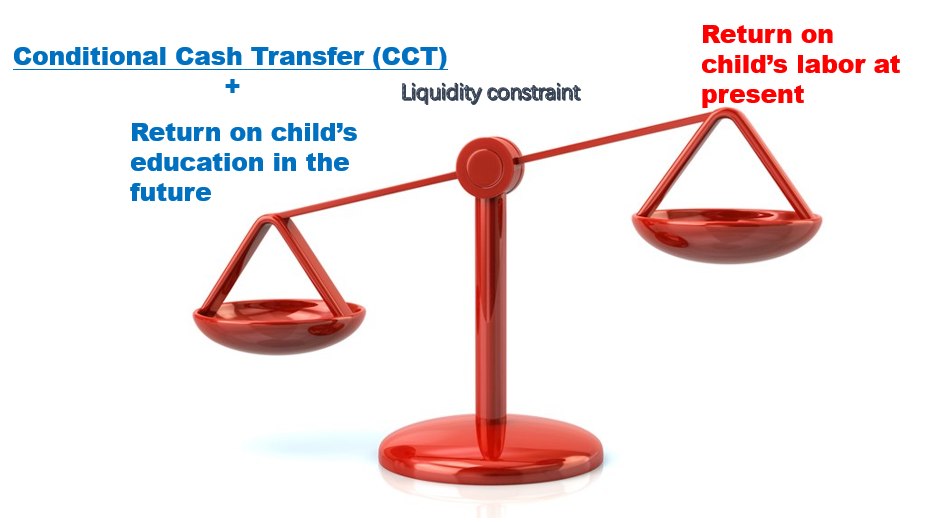
\includegraphics[scale=0.3]{images/balance2.png}
        \label{fig:balance2}
    \end{figure}
    %\pause
    \item The most popular social welfare program in the developing world: over 63 countries have at least one CCT program \textcolor{mygray}{World Bank (2018)}.
\end{itemize}
\end{frame}



%-------------------------------
% \section{Prior Evidence}

\begin{comment}
\begin{frame}
\frametitle{Prior Evidence}

Some studies suggest a positive impact of CCTs on school attendance among:

\begin{itemize}
    \item Marginal children
    \item Larger families where the head of household has a lower educational level
    \item Families with stronger prior willingness to study
\end{itemize}

Other studies show that the increase in school attendance should not be attributed to CCT programs due to the underlying heterogeneity:

\begin{itemize}
    \item Family background
    \item Innate ability
    \item Geographical characteristics
    \item Educational resources
\end{itemize}

\end{frame}
\end{comment}

%---------------------------------------------------------

\begin{comment}
\begin{frame}{Literature Review}

Some studies suggest a \underline{positive} impact of CCTs on school attendance among:

\begin{itemize}
    \item Marginal children
    \item Larger families where the head of household has a lower educational level
    \item Families with stronger prior willingness to study
\end{itemize}

Other studies reveal \underline{insignificant} impacts and argue that the significant results should be be explained by an underlying heterogeneity among beneficiaries:

\begin{itemize}
    \item Family background
    \item Innate ability
    \item Willingness to study
    \item Geographical characteristics
\end{itemize}

\end{frame}
\end{comment}


%---------------------------------------------------------

\begin{frame}{Literature Review}

Overview:

\begin{itemize}
    \item Most studies suggest a \underline{positive} relationship between CCTs and school attendance.
    \item Some other studies reveal an \underline{insignificant} impact of CCTs on school attendance.
\end{itemize}

Why there are two different conclusions from these studies:

\begin{itemize}
    \item Family background
    \item Innate ability
    \item Willingness to study
    \item Geographical characteristics
\end{itemize}

\end{frame}

%---------------------------------------------------------

\begin{frame}{Data}
\framesubtitle{Search Strategy}

\begin{itemize}
    \item Search platforms:
    \begin{itemize}
        \item Google Scholar
        \item Web of Science
        \item Citations and references
    \end{itemize}
    \item Keywords:
    \begin{itemize}
        \item \textit{Conditional Cash Transfers AND School Attendance}
        \item \textit{Conditional Cash Transfers AND Education}
        \item \textit{Conditional Cash Transfers AND Schooling}
        \item \textit{Conditional Cash Transfers AND Attendance}
    \end{itemize}
\end{itemize}
    
\end{frame}

%-----------------------------------------------

\begin{frame}{Data}
\framesubtitle{Eligibility Criteria}

\begin{itemize}
    \item \textbf{Variables of interest}: CCTs and school attendance
    \item \textbf{Language}: the paper must be written in English
    \item \textbf{Year of publication}: the paper should be published after 2000
    \item \textbf{Treated subjects}: the estimated effects should cover at least part of the age range between 11 and 16 years old as affected group
    \item \textbf{Measure of effect}: the reported effect should be measured as percentage changes
    \item \textbf{Standard error}: SE of the estimate should be obtainable
    \item \textbf{Independence}: all the studies should be independent of each other.
\end{itemize}

\end{frame}


%------------------------------------------------

\begin{frame}{Data}
\framesubtitle{Selected Studies}


\begin{table}[!htbp]
    \scriptsize
    \centering
    \begin{tabular}{ lll } 
    \hline\hline
    \textbf{Effect} & \textbf{Study} \\
    \hline
    \multirow{6}{6em}{Positive} 
    & Akresh et al (2013)             \\ 
    & Barrera-Osorio et al (2008)     \\ 
    & Edo et al. (2017)               \\ 
    & Filmer \& Schady (2010)         \\ 
    & Levy \& Ohls (2010)             \\ 
    & Perova \& Vakis (2012)          \\ 
    \hline
    \multirow{4}{4em}{Insignificant} 
    & Armand \& Carneiro (2018)       \\ 
    & Borraz \& Gonzalez (2009)       \\ 
    & Corrales-Herrero et al. (2020)  \\ 
    & Ferre \& Sharif (2014)          \\ 
    \hline\hline
    \end{tabular}
%    \caption{A summary of selected studies}
%    \label{tab:my_label}
\end{table}

\begin{itemize}
    \item Aggregate effect across different genders
    \item Aggregate effect across different age groups
    \item Aggregate effect across different regions
\end{itemize}

\end{frame}



%------------------------------------------------
% \section{Results}


\begin{frame}{Results}
\framesubtitle{Forest Plot}
\begin{center}
\begin{figure}
    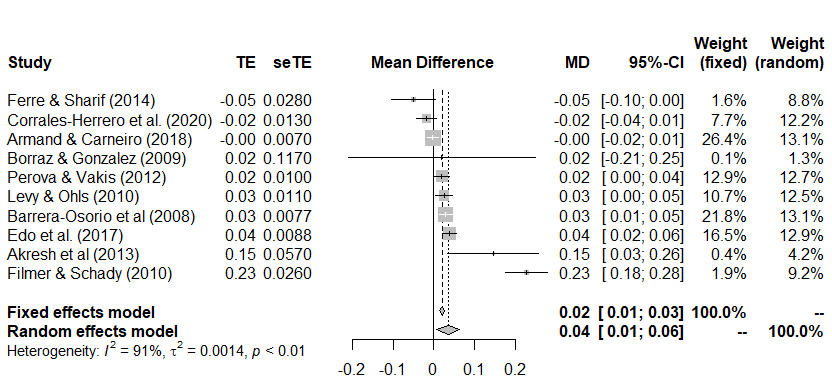
\includegraphics[scale=0.48]{figures/forest_plot.png}
    \label{fig:forest}
\end{figure}
\end{center}
\begin{itemize}
    \item Significantly positive estimates
    \item High heterogeneity: Different implementations of CCTs, country dependant effects, time factors
\end{itemize}
\end{frame}

%------------------------------------------------

% \section{Publication Bias}

\begin{frame}{Publication Bias}
\framesubtitle{Funnel plot}
    \begin{figure}
        \centering
        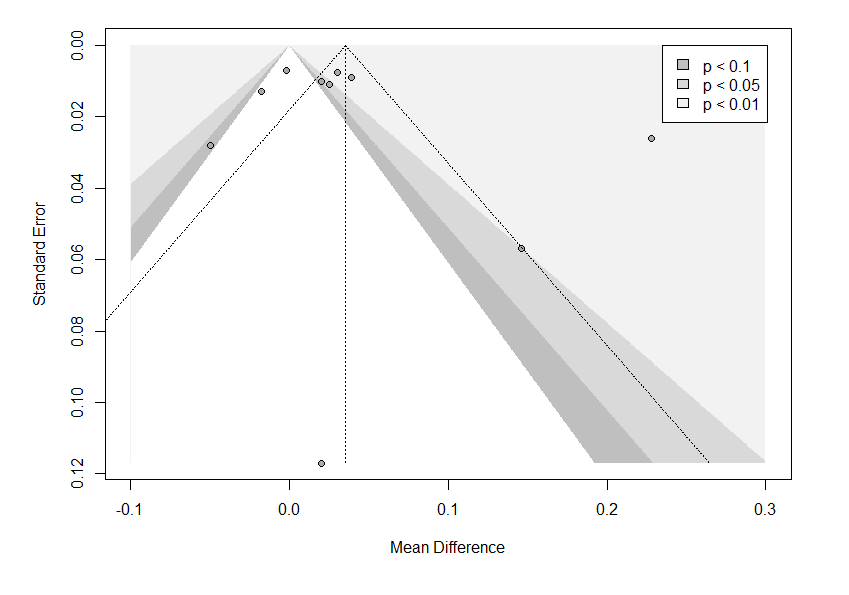
\includegraphics[scale=0.4]{figures/funnel.png}
        \label{fig:funnel}
    \end{figure}
\begin{itemize}
    \item The results appear to be randomly distributed around the random-effects estimator
\end{itemize}
\end{frame}

\begin{frame}{Publication Bias}
\framesubtitle{$t$-statistic}
\begin{figure}
    \centering
    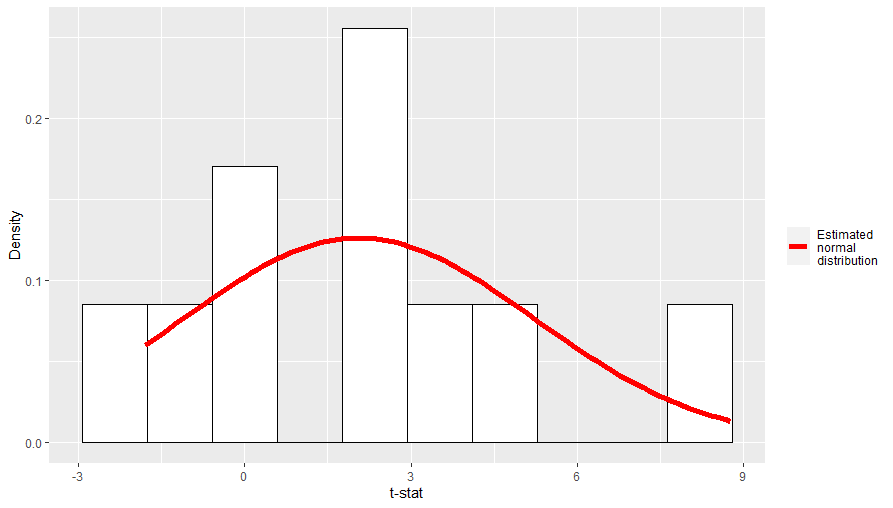
\includegraphics[scale=0.4]{figures/tstat_distribution.png}
    \label{fig:tstat}
\end{figure}
\begin{itemize}
    \item Mean $\approx 2$; SD $\approx 3$
    \item Interesting peak, but large standard deviation
\end{itemize}
\end{frame}

\begin{frame}{Publication Bias}
\framesubtitle{Reported Effects and Standard Errors}
    \begin{figure}
        \centering
        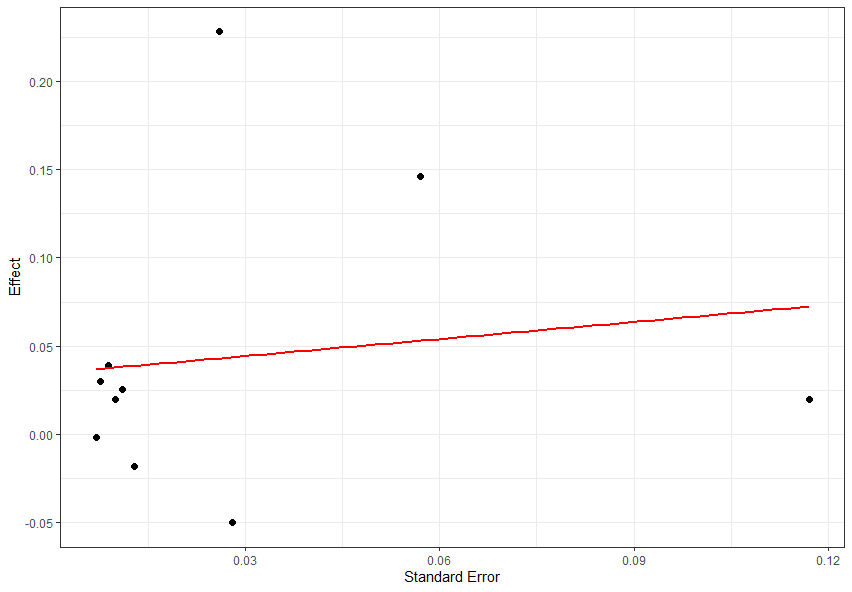
\includegraphics[scale=0.3]{figures/se_effect.png}
        \label{fig:effectse}
    \end{figure}
    \begin{itemize}
        \item No evident correlation
        \item Insignificant estimate of the slope coefficient in a linear regression
    \end{itemize}
\end{frame}


%------------------------------------------------

% \section{Heterogeneity (\& Bias)}

\begin{frame}{Heterogeneity (\& Publication Bias)}
\framesubtitle{Meta-Regression Model}
    $$ReportedEffect_i = \beta_0 + \beta_1 SouthAmerica_i + \beta_2 after2012_i + \beta_3 SE_i + \varepsilon_i$$
    \begin{itemize}
    \item $ReportedEffect_i$ is the a study's reported effect
        \item $\beta_0$ is the estimated underlying effect
        \item $SouthAmerica_i$ is a dummy for studies in South America
        \item $after2012_i$ is a dummy for studies published after 2012
        \item $SE_i$ is the standard error of the reported effect
    \end{itemize}
\end{frame}

\begin{frame}{Heterogeneity (\& Publication Bias)}
\framesubtitle{Regression Results}
    \begin{table}[!htbp] \centering 
  \label{tab:metaregs} 
  \resizebox{\textwidth}{!}{
\begin{tabular}{@{\extracolsep{5pt}}lccccccc} 
 & \multicolumn{7}{c}{\textit{Dependent variable:}} \\ 
\cline{2-8} 
\\[-1.8ex] & \multicolumn{7}{c}{Effect} \\ 
\\[-1.8ex] & (1) & (2) & (3) & (4) & (5) & (6) & (7)\\ 
\hline \\[-1.8ex] 
 SouthAmerica & 0.047 &  & 0.035 &  & 0.045 &  & 0.033 \\ 
  & (0.053) &  & (0.070) &  & (0.057) &  & (0.075) \\
 after2012 &  & $-$0.042 & $-$0.021 &  &  & $-$0.039 & $-$0.020 \\ 
  &  & (0.053) & (0.070) &  &  & (0.057) & (0.075) \\
 SE &  &  &  & 0.322 & 0.211 & 0.218 & 0.187 \\ 
  &  &  &  & (0.830) & (0.862) & (0.873) & (0.931) \\
 RealEffect & 0.020 & 0.065 & 0.037 & 0.035 & 0.015 & 0.057 & 0.031 \\ 
  & (0.037) & (0.038) & (0.068) & (0.036) & (0.044) & (0.050) & (0.079) \\
\hline \\[-1.8ex] 
Observations & 10 & 10 & 10 & 10 & 10 & 10 & 10 \\ 
\hline 
\hline \\[-1.8ex] 
\textit{Note:}  & \multicolumn{7}{r}{$^{*}$p$<$0.1; $^{**}$p$<$0.05; $^{***}$p$<$0.01} \\ 
\end{tabular}}
\end{table}
\end{frame}

%------------------------------------------------
% \section{Conclusion}

\begin{frame}
\frametitle{Conclusion}
\begin{itemize}
    \item Estimated positive significant effect (4 percentage points increase due to CCTs in the random-effects model)
    \item No strong evidence for publication bias
    \item Results to be taken with a grain of salt:
    \begin{itemize}
        \item Small sample size
        \item Heterogeneity remains unaddressed
    \end{itemize}
\end{itemize}



\end{frame}

\begin{frame}
\begin{center}
\begin{huge}
Thank you for your attention!

\vspace{4mm}
Any questions?
\end{huge}

\end{center}


\end{frame}
%------------------------------------------------
%\section{Critics}

%\begin{frame}
%\frametitle{Critics}
    
%\end{frame}




%-------------------------------------------------
%\section{Discussion}

%\begin{frame}
%\frametitle{Discussion}





%\end{frame}

%------------------------------------------------


%----------------------------------------------------------------------------------------

\end{document}